

\tikzset{every picture/.style={line width=0.75pt}} %set default line width to 0.75pt        

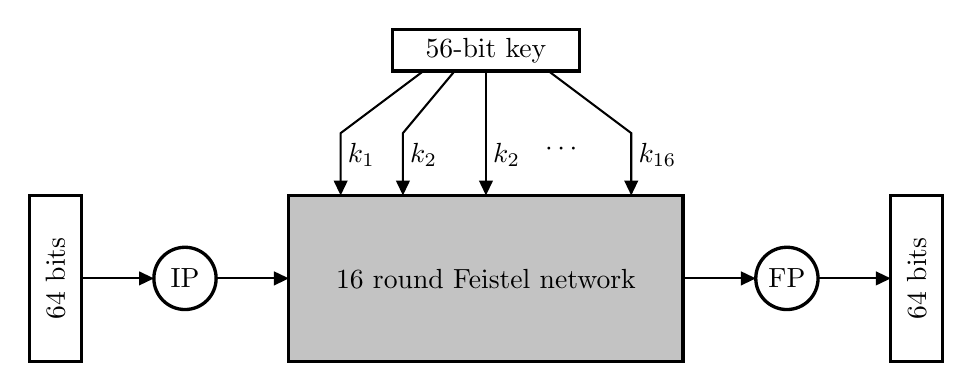
\begin{tikzpicture}[x=0.75pt,y=0.75pt,yscale=-1,xscale=1]
%uncomment if require: \path (0,169); %set diagram left start at 0, and has height of 169

%Shape: Rectangle [id:dp9082761089513578] 
\draw  [line width=1.2]  (0,80) -- (25,80) -- (25,160) -- (0,160) -- cycle ;
%Shape: Circle [id:dp03697940656912868] 
\draw  [line width=1.2]  (60,120) .. controls (60,111.72) and (66.72,105) .. (75,105) .. controls (83.28,105) and (90,111.72) .. (90,120) .. controls (90,128.28) and (83.28,135) .. (75,135) .. controls (66.72,135) and (60,128.28) .. (60,120) -- cycle ;
%Straight Lines [id:da7967662847402655] 
\draw    (25,120) -- (57,120) ;
\draw [shift={(60,120)}, rotate = 180] [fill={rgb, 255:red, 0; green, 0; blue, 0 }  ][line width=0.08]  [draw opacity=0] (7.14,-3.43) -- (0,0) -- (7.14,3.43) -- cycle    ;
%Straight Lines [id:da25423668245796893] 
\draw    (90,120) -- (122,120) ;
\draw [shift={(125,120)}, rotate = 180] [fill={rgb, 255:red, 0; green, 0; blue, 0 }  ][line width=0.08]  [draw opacity=0] (7.14,-3.43) -- (0,0) -- (7.14,3.43) -- cycle    ;
%Shape: Rectangle [id:dp8561305938166983] 
\draw  [fill={rgb, 255:red, 155; green, 155; blue, 155 }  ,fill opacity=0.6 ][line width=1.2]  (125,80) -- (315,80) -- (315,160) -- (125,160) -- cycle ;
%Shape: Circle [id:dp9835625221389512] 
\draw  [line width=1.2]  (350,120) .. controls (350,111.72) and (356.72,105) .. (365,105) .. controls (373.28,105) and (380,111.72) .. (380,120) .. controls (380,128.28) and (373.28,135) .. (365,135) .. controls (356.72,135) and (350,128.28) .. (350,120) -- cycle ;
%Straight Lines [id:da9164504674846901] 
\draw    (315,120) -- (347,120) ;
\draw [shift={(350,120)}, rotate = 180] [fill={rgb, 255:red, 0; green, 0; blue, 0 }  ][line width=0.08]  [draw opacity=0] (7.14,-3.43) -- (0,0) -- (7.14,3.43) -- cycle    ;
%Straight Lines [id:da18967570450355176] 
\draw    (380,120) -- (412,120) ;
\draw [shift={(415,120)}, rotate = 180] [fill={rgb, 255:red, 0; green, 0; blue, 0 }  ][line width=0.08]  [draw opacity=0] (7.14,-3.43) -- (0,0) -- (7.14,3.43) -- cycle    ;
%Shape: Rectangle [id:dp048056129270156456] 
\draw  [line width=1.2]  (415,80) -- (440,80) -- (440,160) -- (415,160) -- cycle ;
%Shape: Rectangle [id:dp764035049296157] 
\draw  [line width=1.2]  (175,0) -- (265,0) -- (265,20) -- (175,20) -- cycle ;
%Straight Lines [id:da0759384102778824] 
\draw    (190,20) -- (150,50) -- (150,77) ;
\draw [shift={(150,80)}, rotate = 270] [fill={rgb, 255:red, 0; green, 0; blue, 0 }  ][line width=0.08]  [draw opacity=0] (7.14,-3.43) -- (0,0) -- (7.14,3.43) -- cycle    ;
%Straight Lines [id:da5205997190861071] 
\draw    (205,20) -- (180,50) -- (180,77) ;
\draw [shift={(180,80)}, rotate = 270] [fill={rgb, 255:red, 0; green, 0; blue, 0 }  ][line width=0.08]  [draw opacity=0] (7.14,-3.43) -- (0,0) -- (7.14,3.43) -- cycle    ;
%Straight Lines [id:da9579629636144731] 
\draw    (220,20) -- (220,77) ;
\draw [shift={(220,80)}, rotate = 270] [fill={rgb, 255:red, 0; green, 0; blue, 0 }  ][line width=0.08]  [draw opacity=0] (7.14,-3.43) -- (0,0) -- (7.14,3.43) -- cycle    ;
%Straight Lines [id:da7033655636977068] 
\draw    (250,20) -- (290,50) -- (290,77) ;
\draw [shift={(290,80)}, rotate = 270] [fill={rgb, 255:red, 0; green, 0; blue, 0 }  ][line width=0.08]  [draw opacity=0] (7.14,-3.43) -- (0,0) -- (7.14,3.43) -- cycle    ;

% Text Node
\draw (12.5,120) node  [rotate=-270] [align=left] {$\displaystyle 64$ bits};
% Text Node
\draw (427.5,120) node  [rotate=-270] [align=left] {$\displaystyle 64$ bits};
% Text Node
\draw (220,120) node   [align=left] {$\displaystyle 16$ round Feistel network};
% Text Node
\draw (220,10) node   [align=left] {$\displaystyle 56$-bit key};
% Text Node
\draw (75,120) node   [align=left] {IP};
% Text Node
\draw (365,120) node   [align=left] {FP};
% Text Node
\draw (152,53.4) node [anchor=north west][inner sep=0.75pt]    {$k_{1}$};
% Text Node
\draw (182,53.4) node [anchor=north west][inner sep=0.75pt]    {$k_{2}$};
% Text Node
\draw (222,53.4) node [anchor=north west][inner sep=0.75pt]    {$k_{2}$};
% Text Node
\draw (292,53.4) node [anchor=north west][inner sep=0.75pt]    {$k_{16}$};
% Text Node
\draw (247,53.4) node [anchor=north west][inner sep=0.75pt]    {$\cdots $};


\end{tikzpicture}